% The three levels of LVS in a 2.5D assembly.
% Levels 1 and 2 are ordinary PDK LVS. Level 3 is the one the assembly adds.
\documentclass[border=4pt]{standalone}
\usepackage{tikz}
\usetikzlibrary{arrows.meta, positioning, calc, fit}
\usepackage[T1]{fontenc}
\usepackage{lmodern}

% Hyphen breaks inside the small figure labels read badly.
\hyphenpenalty=10000
\exhyphenpenalty=10000

\definecolor{IHPfg}{RGB}{0,80,139}
\definecolor{IHPaccent}{RGB}{109,112,114}

\begin{document}
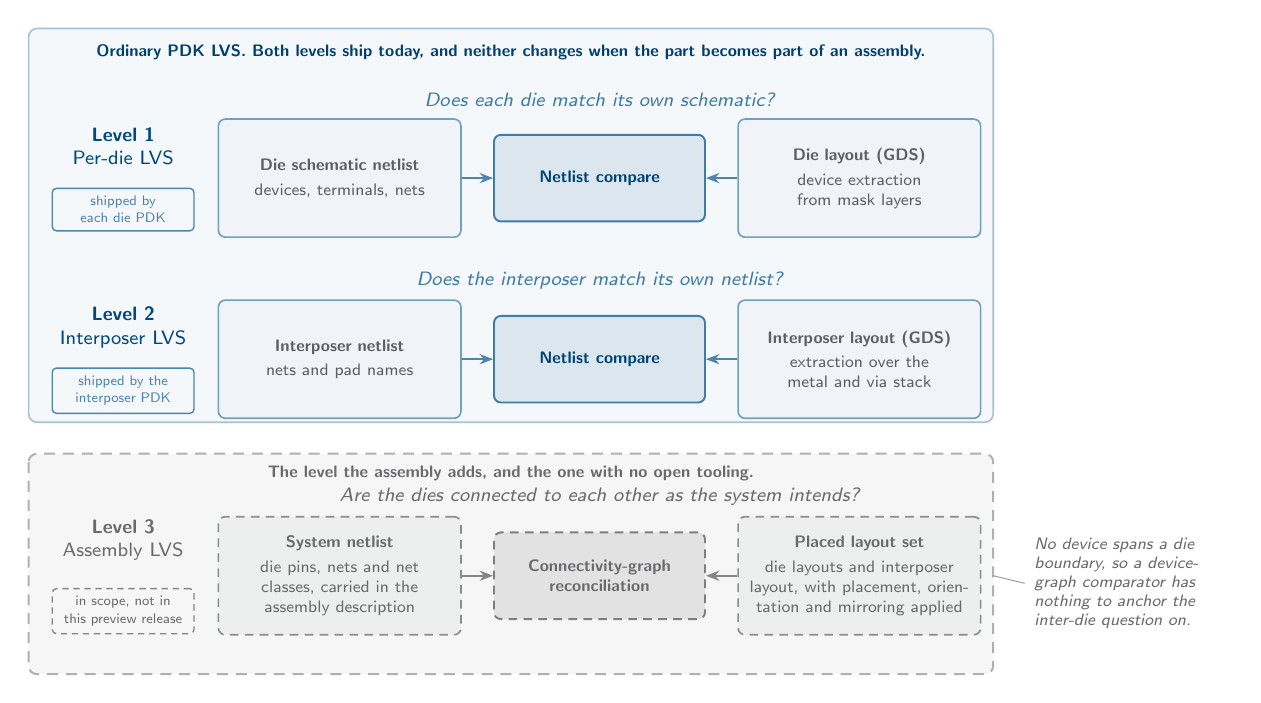
\begin{tikzpicture}[
    x=1mm, y=1mm,
    >=Stealth,
    adkside/.style={
        rectangle, rounded corners=2.5pt,
        draw=IHPfg!55, fill=IHPfg!6, line width=0.6pt,
        text width=28mm, minimum height=15mm,
        font=\sffamily\fontsize{6}{7.2}\selectfont, text=IHPaccent!85!black,
        align=center, inner sep=1.4mm
    },
    adkcomp/.style={
        rectangle, rounded corners=2.5pt,
        draw=IHPfg!75, fill=IHPfg!14, line width=0.7pt,
        text width=24mm, minimum height=11mm,
        font=\sffamily\fontsize{6.2}{7.4}\selectfont\bfseries, text=IHPfg!85!black,
        align=center, inner sep=1.4mm
    },
    adksidedash/.style={
        rectangle, rounded corners=2.5pt,
        draw=IHPaccent!80, fill=IHPaccent!12, line width=0.6pt, dashed, dash pattern=on 1.1mm off 0.8mm,
        text width=28mm, minimum height=15mm,
        font=\sffamily\fontsize{6}{7.2}\selectfont, text=IHPaccent!95!black,
        align=center, inner sep=1.4mm
    },
    adkcompdash/.style={
        rectangle, rounded corners=2.5pt,
        draw=IHPaccent!90, fill=IHPaccent!20, line width=0.7pt, dashed, dash pattern=on 1.1mm off 0.8mm,
        text width=24mm, minimum height=11mm,
        font=\sffamily\fontsize{6.2}{7.4}\selectfont\bfseries, text=IHPaccent!95!black,
        align=center, inner sep=1.4mm
    },
    adklevel/.style={
        text width=19mm, align=center,
        font=\sffamily\fontsize{7}{8.4}\selectfont, text=#1
    },
    adkbadge/.style={
        rectangle, rounded corners=1.5pt,
        draw=#1, line width=0.5pt,
        text width=16mm, align=center, inner sep=1mm,
        font=\sffamily\fontsize{5.2}{6.2}\selectfont, text=#1
    },
    adkbadgedash/.style={
        rectangle, rounded corners=1.5pt,
        draw=IHPaccent!85, line width=0.5pt, dashed, dash pattern=on 0.8mm off 0.6mm,
        text width=16mm, align=center, inner sep=1mm,
        font=\sffamily\fontsize{5.2}{6.2}\selectfont, text=IHPaccent!95!black
    },
    adkask/.style={
        font=\sffamily\fontsize{6.6}{8}\selectfont\itshape, text=#1, align=center
    },
    adkgroup/.style={
        text width=110mm, align=center,
        font=\sffamily\fontsize{6.2}{7.4}\selectfont\bfseries, text=#1
    },
    adkarrow/.style={
        -{Stealth[length=1.7mm, width=1.3mm]}, line width=0.6pt, color=#1
    },
    adknote/.style={
        text width=24mm, align=left,
        font=\sffamily\fontsize{5.6}{6.8}\selectfont\itshape, text=IHPaccent!95!black
    }
]

% ===== Group A backdrop: the two levels that are ordinary PDK LVS =====
\fill[IHPfg!4, rounded corners=3pt] (-2.5,9) rectangle (120,-41);
\draw[IHPfg!35, line width=0.6pt, rounded corners=3pt] (-2.5,9) rectangle (120,-41);

\node[adkgroup=IHPfg!80!black] at (58.75, 6)
    {Ordinary PDK LVS. Both levels ship today, and neither changes when the part
     becomes part of an assembly.};

% ===== Group B backdrop: the level the assembly adds =====
\fill[IHPaccent!6, rounded corners=3pt] (-2.5,-45) rectangle (120,-73);
\draw[IHPaccent!55, line width=0.7pt, dashed, dash pattern=on 1.4mm off 1mm,
      rounded corners=3pt] (-2.5,-45) rectangle (120,-73);

\node[adkgroup=IHPaccent!95!black] at (58.75, -47.5)
    {The level the assembly adds, and the one with no open tooling.};

% ===== Level 1: per-die LVS =====
\node[adkask=IHPfg!75] at (70, 0) {Does each die match its own schematic?};

\node[adklevel=IHPfg!90!black] at (9.5, -6)
    {\textbf{Level 1}\\Per-die LVS};
\node[adkbadge=IHPfg!70] at (9.5, -14) {shipped by each die PDK};

\node[adkside] (r1) at (37, -10)
    {\textbf{Die schematic netlist}\\[0.6mm]devices, terminals, nets};
\node[adkcomp] (c1) at (70, -10) {Netlist compare};
\node[adkside] (i1) at (103, -10)
    {\textbf{Die layout (GDS)}\\[0.6mm]device extraction from mask layers};

\draw[adkarrow=IHPfg!70] (r1.east) -- (c1.west);
\draw[adkarrow=IHPfg!70] (i1.west) -- (c1.east);

% ===== Level 2: interposer LVS =====
\node[adkask=IHPfg!75] at (70, -23) {Does the interposer match its own netlist?};

\node[adklevel=IHPfg!90!black] at (9.5, -29)
    {\textbf{Level 2}\\Interposer LVS};
\node[adkbadge=IHPfg!70] at (9.5, -37) {shipped by the interposer PDK};

\node[adkside] (r2) at (37, -33)
    {\textbf{Interposer netlist}\\[0.6mm]nets and pad names};
\node[adkcomp] (c2) at (70, -33) {Netlist compare};
\node[adkside] (i2) at (103, -33)
    {\textbf{Interposer layout (GDS)}\\[0.6mm]extraction over the metal and via stack};

\draw[adkarrow=IHPfg!70] (r2.east) -- (c2.west);
\draw[adkarrow=IHPfg!70] (i2.west) -- (c2.east);

% ===== Level 3: assembly LVS, scope only =====
\node[adkask=IHPaccent!95!black] at (70, -50.5)
    {Are the dies connected to each other as the system intends?};

\node[adklevel=IHPaccent!95!black] at (9.5, -56)
    {\textbf{Level 3}\\Assembly LVS};
\node[adkbadgedash] at (9.5, -65) {in scope, not in this preview release};

\node[adksidedash] (r3) at (37, -60.5)
    {\textbf{System netlist}\\[0.6mm]die pins, nets and net classes, carried in the assembly description};
\node[adkcompdash] (c3) at (70, -60.5) {Connectivity-graph reconciliation};
\node[adksidedash] (i3) at (103, -60.5)
    {\textbf{Placed layout set}\\[0.6mm]die layouts and interposer layout, with placement, orientation and mirroring applied};

\draw[adkarrow=IHPaccent!85] (r3.east) -- (c3.west);
\draw[adkarrow=IHPaccent!85] (i3.west) -- (c3.east);

% Callout on the missing anchor for device-graph comparison
\node[adknote, anchor=north west] (note) at (124, -54.5)
    {No device spans a die boundary, so a device-graph comparator has nothing
     to anchor the inter-die question on.};

\draw[IHPaccent!70, line width=0.35pt] (note.west) -- ([xshift=1.5mm]i3.east);

\end{tikzpicture}
\end{document}
